% !TEX root = ../main.tex

\section{前言：巢湖绿韵}
\subsection{研究背景}
环巢湖湿地是长江经济带"共抓大保护"战略中的关键生态节点，亦是巢湖流域生态安全的"核心屏障"。作为湖泊与陆地的过渡带，其植被群落（挺水植物芦苇、浮叶植物菱、沉水植物菹草等）通过发达根系固岸御浪、繁茂茎叶净化水体、复杂结构庇护生灵，构建了"水陆共生"的生态系统基础。据《安徽省湿地保护公报（2024）》数据\cite{chu2023}，环巢湖湿地总面积达12.7万公顷，占巢湖流域湿地总面积的68\%，其中植被覆盖区贡献了流域70\%以上的氮磷拦截量与50\%的淡水碳汇，对维系巢湖水质稳定与流域生态平衡具有不可替代的作用，\autoref{tab:chaohu-wetlands-simplified}为环巢湖十大湿地（十八联圩、巢湖半岛等）的基本信息，\autoref{fig:wetland-area-ratio}为环巢湖十大湿地的面积比例关系。
\begin{table}[htbp]
\centering
\caption{环巢湖十大湿地基本信息（截至2024年）}
\label{tab:chaohu-wetlands-simplified}
\begin{tabular}{lccc}
\toprule
\textbf{湿地名称} & \textbf{位置} & \textbf{面积（公顷）} & \textbf{主要特色} \\
\midrule
巢湖湖滨湿地 & 包河区巢湖北岸 & 1535.31 & 浮游生物多 \\
肥西三河湿地 & 肥西县三河镇 & 1887.22 & 保护植物集中 \\
巢湖半岛湿地 & 巢湖市中庙街道/黄麓镇 & 998.36 & 红杉林显著 \\
巢湖槐林湿地 & 巢湖市槐林镇 & 193.96 & 原生芦苇多 \\
巢湖柘皋河湿地 & 巢湖市柘皋镇 & 446.65 & 河道修复，"杉影花海" \\
肥东十八联圩湿地 & 肥东县长临河镇 & 2760.00 & 净化功能强 \\
肥东玉带河湿地 & 肥东县长临河镇 & 41.40 & 微型湿地，净化径流 \\
庐江栖凤洲湿地 & 庐江县同大镇 & 843.53 & 原始滩涂 \\
庐江马尾河湿地 & 庐江县盛桥镇 & 857.20 & 沉水植物修复 \\
包河派河口湿地 & 包河区派河镇 & 239.67 & "水下森林"示范 \\
\bottomrule
\end{tabular}
\footnotesize{注：数据综合自合肥市林园局、巢湖研究院公开资料（2024）。}
\end{table}

\begin{figure}[htbp]
    \centering
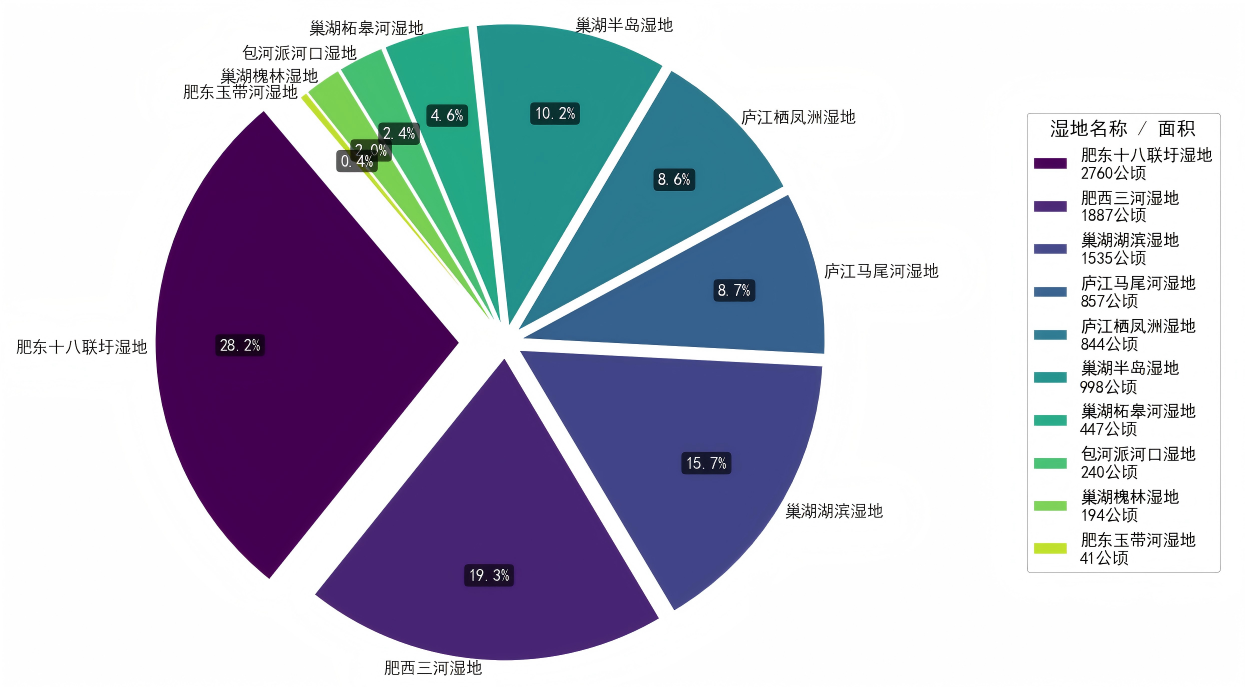
\includegraphics[width=1\linewidth]{img/十大湿地.png}
    \caption{环巢湖十大湿地面积比例关系}
    \label{fig:wetland-area-ratio}
\end{figure}

近年来，随着环巢湖十大湿地生态修复工程的推进，局部植被生态得到显著改善，生态修复成效如\autoref{fig:restoration-effectiveness}所示：
\begin{figure}[htbp]
    \centering
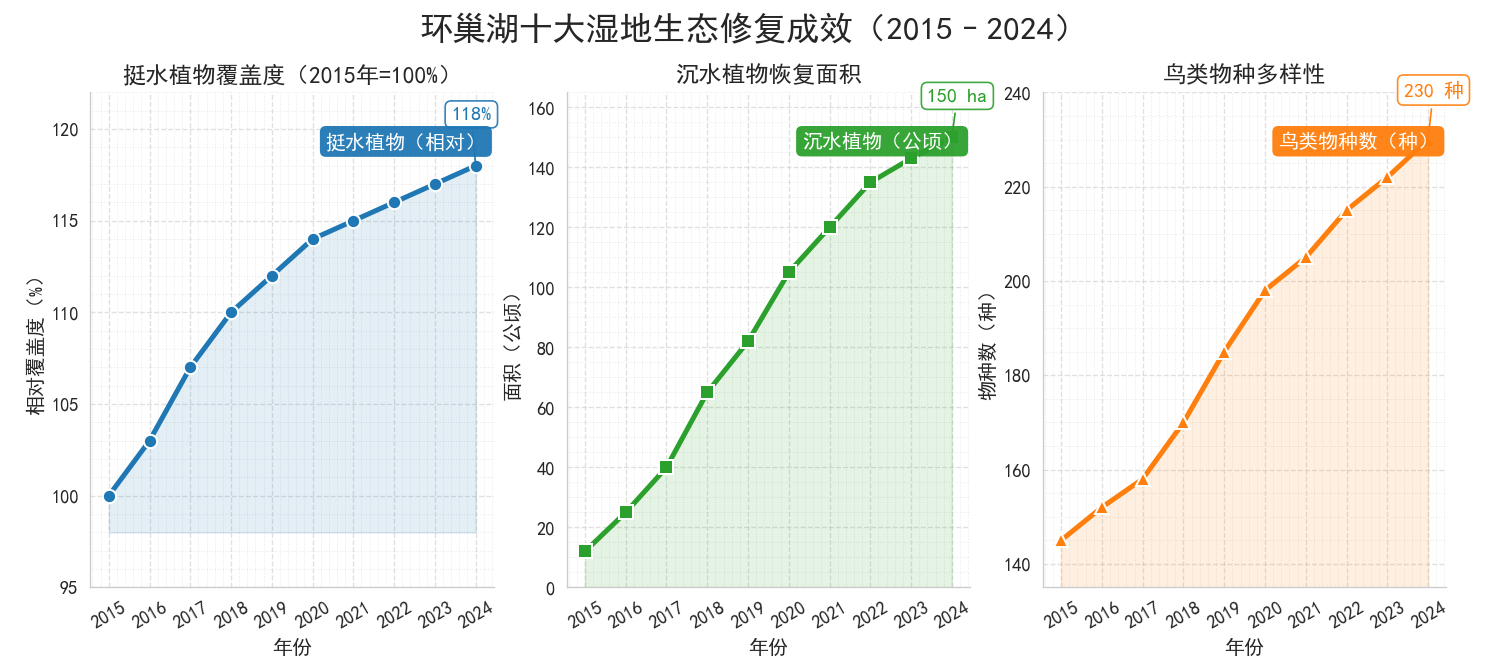
\includegraphics[width=1\linewidth]{img/Figure_2.png}
    \caption{环巢湖十大湿地生态修复成效}
    \label{fig:restoration-effectiveness}
\end{figure}

从\autoref{fig:restoration-effectiveness}中可以看出，截至2024年，核心区挺水植物覆盖度较2015年提升18\%，沉水植物在半岛湿地等区域恢复面积达150公顷，鸟类多样性增至230种（较2018年增长35\%）\cite{tang2022}。

但从流域尺度看，湿地植被仍面临多重困境，生态系统脆弱性凸显，具体有如下表现：

\subsubsection{水文节律紊乱导致植被生境退化}
巢湖自1962年建闸后失去自然季节性水位波动特征，年际水位变幅达2-3米，打破了植被"淹水-落干"的自然适应周期。一方面，西岸中庙街道湖滩的芦苇群落因长期高水位浸泡，根系缺氧腐烂，近十年面积缩减40\%，植被带向陆地方向退缩150-200米；另一方面，枯水期水位过低（低于8.0米）导致烔炀河入湖口湿生草甸干旱化，稗草等耐旱物种挤占原生虉草生境，湿生植被群落多样性下降27\%\cite{liu2022}。

\subsubsection{水体污染加剧植被群落衰退}
周边农业面源污染（20万亩农田年均化肥流失量约1.2万吨）与城市生活污水（合肥、巢湖市日均排污量约50万吨）持续输入，导致巢湖西半湖总氮（TN）浓度常年维持在1.5-2.0mg/L（超V类水质标准3-4倍），水体透明度从2010年的1.2米降至2024年的0.6米\cite{yao2022}。沉水植物因光照不足，分布下限从3米水深退缩至1.5米，菹草、苦草等清洁水体指示物种在西湖心区域近乎消失，取而代之的是耐污物种微齿眼子菜的单一化扩张，群落结构趋于简化。

\subsubsection{外来物种入侵挤压本土植被空间}
喜旱莲子草、凤眼莲（水葫芦）在派河河口、槐林湿地等静水区域疯狂扩张，其中凤眼莲入侵面积已达300公顷，形成单一"绿色荒漠"。监测数据显示，入侵区域本土植物种类从2018年的18种降至2024年的7种，生物多样性指数下降61\%\cite{luwen2022}；且死亡植株分解释放的氮磷量占该区域外源污染的25\%，形成"污染-入侵-再污染"的恶性循环，进一步抑制本土植被生长。

\subsubsection{生境破碎化割裂植被生态连通性}
城市化与基础设施建设导致湿地景观严重割裂：巢湖东岸开发区建设中，道路、房地产项目将原本连续的湖滨植被带切割为12个孤立片段，植被连通性指数从2015年的0.72降至2024年的0.39；历史围垦养殖（累计围垦面积达1.2万公顷）导致湿地核心生境丧失，湿生草甸面积较2000年减少58\%\cite{zhou2024}，无法为迁徙鸟类提供连续的觅食与栖息廊道。

当前，环巢湖湿地正面临"生态保护与区域发展"的核心矛盾：一方面，作为巢湖富营养化治理的关键环节，湿地植被需承担更重的生态净化任务；另一方面，周边农业生产、生态旅游等人类活动对植被生境的干扰持续增强。在此背景下，系统剖析环巢湖湿地植被的群落结构规律、量化其生态功能价值、诊断关键威胁因子并提出科学可行的保护修复策略，不仅能为巢湖流域"十四五"生态治理提供实践依据，更可为长江中下游淡水湖滨湿地（如鄱阳湖、洞庭湖）的"植被修复-生态维稳-可持续利用"提供典型范式，具有重要的生态、经济与社会意义。

\subsection{研究思路}
本文以"数据驱动-机制解析-策略落地"为核心逻辑，围绕环巢湖湿地植被"结构-功能-威胁-修复"四大核心议题，构建"实地调查+遥感解译+量化分析+策略验证"的研究框架，具体步骤如下：
